\documentclass[nocrop]{bioinfo}
\usepackage{siunitx}
\usepackage{mathtools}
\usepackage{amssymb}
\usepackage{mathrsfs}
\usepackage{physics}
\usepackage{booktabs}
\usepackage[hidelinks]{hyperref}
\usepackage{multirow}
\usepackage{graphicx}
\usepackage{tabularx}
\sisetup{round-precision=3}
\sisetup{round-mode=places, exponent-product=\cdot}
\copyrightyear{} \pubyear{}

\graphicspath{{./images/}}
\access{}
\appnotes{Project Report}

\begin{document}
\firstpage{1}

\subtitle{Project Report}
	
\title[short Title]{Secondary structure prediction: a probabilistic and machine learning showdown}
\author[Roncelli S.]{Roncelli Stefano\,$^{\text{\sfb 1,}*}$}
\address{$^{\text{\sf 1}}$International Master in Bioinformatics, Univerisity of Bologna, Bologna}
\corresp{$^\ast$To whom correspondence should be addressed.}
\history{}
\editor{}
\abstract{\textbf{Motivation:} Protein structure prediction is of paramount importance in many fields. Through the decades many breakthougts allowed to extend the boundaries of sequence based prediction further than the generation before, but still nowhere near structure based methods. Analysis of the most significant innovations is essential in deriving a knowledgebase to devise even powerful methods.\\
		\textbf{Results:} Powerful models allow to model non-linearity. However, the risk of overfitting is always plaguing complex predictors. More simple probabilistic models can yield comparable results if used in an information-rich context.\\
		\textbf{Contact:}\href{stefano.roncelli@studio.unibo.it}{stefano.roncelli@studio.unibo.it}\\
		\textbf{Supplementary information:} Supplementary data are available at github.}
\maketitle
\section{Introduction}
Prediction and pattern recognition is one of the core topics in all bioinformatic fields.
Specifically, secondary structure prediction was first attempted around 60 years ago with analysis on the Helix-Coil transition \citep{Zimm1959} \citep{Lifson1961}, but the lack of available structures hindered the progress.
It was more than a decade later that the first probabilistic models set the start of what we now know as 'first generation' of sequence-based secondary structure prediction.
Their somewhat respectable performances (if we frame the epoque) were limited by the fact that they modeled only the statical propensities on the single residues for the prediction of the secondary structure.
It was only with the second generation that the context \citep{Garnier1978} was taken into account for more accurate predictions, which were verging 60\% accuracy.
This context takes the form of a sliding window centered on the residue for which the effort of predicting its structure resides, but the lack of available known sequences resulted again in difficult estimation of the parameters.
Only when the numbers finally caught up, the third generation models were able to harness the valuable data provided by evolution, in the form of sequence profiles derived from multiple sequence alignments, and breached the 70\% accuracy threshold.
Today, state-of-the-art pushed the threshold even higher \citep{bibid}, even though the theoretical limit of 88\% has not yet been achieved \citep{Rost2001}\citep{Russell1993}.
Thanks to the independent advancements in machine learning, most notably neural networks \citep{Drozdetskiy2015}\citep{Heffernan2018} and Support Vector Machines \citep{Kieslich2016}, the boundary stalls at 82\% accuracy.

Here, we propose a side by side comparison between the old and the new: a performance review between a model based on the time-proven Garnier-Osguthorpe-Robson method \citep{Garnier1978} and a much more modern estimator based on Support Vector Machines \citep{Cortes1995}.
All steps from dataset preparation, to profile generation, to scoring have been devised in order to compare their performances on equal grounds. 
Such datasets are designed to represent as accurately as possible the protein space, albeit with some simplifications.
This review is motivated by the curiosity to asses the peculiarities and differences of the two approaches. 

%\enlargethispage{12pt}
\begin{methods}
\section{Methods}
\subsection{Training set preparation}
The training set contains \num{1348} protein primary and secondary sequences in fasta format as available from JPred4 \citep{Drozdetskiy2015}.
For correct class identification, the \textit{de facto} golden standard is the labeling of residues based on the three dimensional structure, in the form of a structure file such as a macro molecular Christallographic Information File (mmCIF).
This information retrieval of the "true" classes of a chain is usually achieved by Define Secondary Structure of Proteins (DSSP)\citep{Kabsch1983} or STRuctural IDEntification (STRIDE)\citep{frishman1995knowledge} algorithms.

Proteins form a wide variety of secondary structures, however, JPred remaps the eight DSSP's categories with a three state notation: $\alpha$-helices (H) are labeled as H, beta strands (E) and residues in $\beta$-bridge (B) as E, and everything else as C. 
Hence, all the possible structures can be either labeled as helix (H), extended strand (E) or coil (C).
It is important to note that whereas the H and E classes maintain a certain degree of homogeneity, the C category is more spurious in nature, since it groups together many, widely different, secondary structure conformations.
To be precise, such mapping is a methodological mistake, because afterwards it is no longer possible to distinguish well defined structures (the turns, the 3$_{10}$ helixes and so on) from the errors and limitations of the program (the " " blanks), since they are all collapsed into the C class.
Odd as it may seem, this remapping has the benefit of denoising the two most emblematic classes, alas, at the expense of the Coil category.
In this framework we relate the C category as "not H or E": whatever is not helix or strand is swept under the rug and labeled C.
We will see later how this influences the estimators classification performance.
 
\subsection{Test set}
The JPred dataset comes with a test set, but we decided to generate a new one \textit{de novo}, following the approach of the original JPred test set. 
The RCSB Protein Data Bank (PDB)(\href{rcsb.org}{rcsb.org}) \citep{Berman2000} was queried in order to retrieve all the proteins that met the following criteria:
\begin{itemize}
	\item Deposit date after \date{Jan, 2015}, \textit{i.e.} after the release of JPred4.
	\item Resolution above 2.5\SIUnitSymbolAngstrom: high quality data is important in secondary structure determination when using atomic coodinates. 
	\item Chain length between 50 and 300 residues.
	\item No mutations or artifacts as they may bias the estimators performance.
\end{itemize}
This raw dataset, however, is highly redundant.
Many entries are similar to others in this set or to ones already present in the training set and must be removed.
As a cutoff threshold, we kept only sequences that share less than 30\% sequence identity to other proteins in the test set.
This internal redundancy filtering was achieved by clusterization with MMseqsS \citep{Steinegger2017, Steinegger2018}, with a coverage threshold of 50\%.
To identify the similar proteins between train and test set, the latter was aligned with the former with BLASTp \citep{Altschul1990}. 
To avoid non-significant alignments, an E-value threshold of 0.01 was enforced.
Again, protein recognized to share more than 30\% sequence identity to the training set were purged from the test.
For the generation of the secondary structure annotation we used the same standard as JPred: DSSP.
To be consinstent with JPred's pipeline, the same reduced mapping was used as previously discussed.
The sole difference with the original test set was the elimination of entries whose secondary structure, as determined by DSSP, was shorter than their respective primary structure.
Whereas JPred's approach allows for no more than 9 mismatched between primary and secondary structure, we opted for a no tolerance rule.
 
\subsection{Profile generation}
Using only plain sequences is possible, but complementing it with evolutionary information allows us to achieve much more accurate predictions at virtually no cost.
Following this rationale, each entry in both sets was converted to its relative sequence profile by means of Psiblast \citep{Altschul1997} against the SwissProt as of \texttt{December 2020} \citep{2018a} with the following parameters: e-value set to 0.01, number of descriptions and alignments both set to 10000 and number of iterations equal to 3.
Since the GOR model uses a probabilistic framework to operate, the probabilities in the sequence profiles were normalized accordingly.
For each position in a profile, two windows were extracted, one of size 1 and another of size 17, both centered on the residue of interest.
To avoid inconsistent window length sizes, for the positions at both ends of a profile an adequate amount of padding was introduced, with all values set to 0.
Since all the estimators implemented, by design, work on a vectorized input, each window was then reshaped accordingly and appended to the final dataset.
Through the filtering process, the candidate test set was enormously reduced in size: from more than 12000 candidates we obtained a total of 453 sequence profiles.
To mimic the size of the original test set from JPred, 150 profiles were randomly sampled until their residue and secondary structure composition was comparable to the training set with a tolerance threshold of less than 2\% for secondary structure differences.
Subsamples that did not met the tolerance criteria were discarded and the whole test set resampled.
This ensures that the test set is a valid representative of both the protein space and the training set, so that the performances of the estimators are as unbiased as possible.
\subsection{GOR method}
\subsubsection*{Theorical backround}

The Garnier-Osguthorpe-Robson \citep{Garnier1978} method is a information theory model for secondary structure prediction, and is based on the statical propensities of residues for secondary structure conformations. 
It is possible to devise an information function $I$ that calculates the probability a residue $R$ to be in the conformation $S$, such that:
\begin{equation}
	I(S;R)=\log\frac{P(S|R)}{P(S)}
\end{equation}
Where $P(S|R)$ is the conditional probability of observing residue $R$ in conformation $S$, and $P(S)$ is the probability of conformation $S$.
Using the chain rule:

\begin{equation}
	I(S;R)=\log\frac{P(R,S)}{P(S)P(R)}
\end{equation}

If we want (and we should) also take into consideration the \textit{context} of each residue, that is, how much nearby residues influence the structural conformation of a given R:

\begin{equation}\label{capital}
	I(S, R_{-d},...,R_{d} ) = \log \frac{P(S|R_{-d},...,R_{d})}{P(S)P(R_{-d},...,R_{d} )}
\end{equation}

Where $d$ is the number of residues taken into consideration before and after the central residue.
Training the model therefore consist in the correct estimation of the probabilities involved:
$P(S)$ and $P(R_{-d},...,R_{d})$ are easy to estimate, since for a large enough traning set they can be approximated to their correspondent frequencies.
$P(S|R_{-d},...,R_{d})$, however, is much harder to estimate reliably. 
First and foremost, because it is very computationally challenging due to the exponential increase for wider window sizes.
Second, a good approximation of the true probabilities is very depending of the size of the training set.
For these reasons two simplifying assumptions have to be introduced: the limitation of the window size and the statistical independence of nearby residues.
It is important to note that these assumption are not biologically justifiable, but they help to reshape an untractable problem into a more approachable one.
The size of the window is usually 17, which means:
\begin{equation}
	P(S|R_{-8},...,R_{8}) = \prod_{k=-8}^{8}P(R_k)
\end{equation}
So we can rewrite \eqref{capital} as:
\begin{equation}
	I(S, R_{-8},...,R_{8} ) = \prod_{k=-8}^{8} \log \frac{P(R_k,S)}{P(S)P(R_k)}
\end{equation}
For a large enough training set the probabilities can be approximated to their correspondent frequencies.
Usually the trained model takes the form of an information table or matrix, which is filled according to the frequencies derived from the training set.
In this probabilistic framework, predicting the secondary structure of an unknown sequence $S^*$ means labeling each position with the highest class probability, which is another level over-simplification of the model:
\begin{equation}
	S^* = \arg \max_S  I(S, R_{-8},...,R_{8} )
\end{equation}

\subsubsection*{Implementation}
To test for the context contribution, two models were trained: one with the window size set to 1 (\textit{i.e.} no context) and another with the window set to 17.
As previously discussed, our practical implementation revolves around the use of sequence profiles to boost the estimator performance.
Especially for the GOR, which makes some hindering simplifying assumptions, this proves to be a significant boon to the information content of the training set, which somewhat counterbalances the information loss caused by the model assumptions.
Our implementation of the GOR method starts from the appropriate reshaping of the vectorized sample of the training set.
The information is then stored in an intuitive manner: specifically, a dictionary of NumPy arrays \citep{harris2020array}.
Training the model proceeds in a top-down fashion, iteratively reshaping all the windows of the training dataset.
After that, the appropriate parameters are estimated following the just discussed rationale.
Prediction is as straight-forward as fitting the estimator: for each profile window the estimation of the probabilities is computed from the fitted estimator.
In the event of ties, such as when a specific window contains no signal, the estimator defaults to C class prediction.
This bias is justified by the reduced mapping introduced for the classes.

\subsection{SVM model}
\subsubsection*{Theoretical background}
Support vector machines \citep{Cortes1995} are a class of supervised learning models used both for classification and regression tasks.
At their core reside the computation of a maximum margin hyperplane that is able to separate two classes.
An hyperplane is a N-1 dimensional manifold, where N is the dimension of the feature space, an can be formulated as: 
\begin{equation}
	\vb{w}^T\vb{x}+b=0
\end{equation}
Where $\vb{w}$ is a vector perpendicular to the hyperplane, $\vb{x}$ any point that lies on the hyperplane, and $b$ is a bias to unbound hyperplanes from passing through the origin.
By definition, such hyperplane divides the space in two subspaces, one for each class.
Formally:
\begin{equation}\label{separation}
	t_n(\vb{w}^T\vb{x}+b) \geq 1
\end{equation}
Where $t_n$ is the target variable (the class).
Equation \eqref{separation} states all the points must lie on correct side of the subspace.
The margin $\rho$ can be seen as the distance between two parallel hyperplanes and is:
\begin{equation}\label{margin}
	\rho = \frac{2}{\norm{\vb{w}}}
\end{equation}
The problem of minimazation of the margin hence can be expressed as:
\begin{equation}
	\arg\min_{\vb{w}, b}  \frac{1}{2} \norm{\vb{w}}^2
\end{equation}
We can therefore formulate the original problem as the minimization of \eqref{margin}, subject to \eqref{separation}, which is a constrained optimization problem.
The classical approach involves the use Lagrange multipliers in conjunction with Karush-Kuhn-Tucker \citep{Karush} conditions:
\begin{equation}\label{lagrangian}
	\mathcal{L}(\vb{w},b,\vb{a}) = \frac{1}{2}\norm{\vb{w}}^2 + \sum_n a_n [1 - t_n(\vb{w}^T\vb{x} + b)]
\end{equation}
\eqref{lagrangian} is function of $\vb{w}$, $b$ and $\vb{a}$, but it can be rewritten as a function of $\vb{a}$, the \textit{dual lagrangian}:
\begin{equation}\label{dual}
	\mathcal{\widetilde{L}}(\vb{a}) = \sum_n a_n - \frac{1}{2}\sum_n \sum_m a_n a_m t_n t_m \langle\vb{x}_n \vb{x}_m\rangle 
\end{equation}
subject to
\begin{align}
		&\sum_n a_n t_n = 0 
		&a_n \geq 0 \
\end{align}
Which is a quadratic optimization problem of a convex function, and therefore allows to find a global optimum.
So far, this framework allows only to tackle linearly separable problems.
To extend SVMs beyond linear separation, two methods have been successfully implemented.
The first, easier, approach is to allow some degree of misclassification of the model by relaxing the margins. 
This is achieved with the introduction of $\xi$, a \textit{slack variable}, that changes \eqref{separation} and \eqref{margin} in:
\begin{align}
	&t_n y(\vb{x}) \geq 1 - \xi_n
    &C \sum_n \xi_n + \frac{1}{2}\norm{\vb{w}}^2
\end{align}
This means that now it is possible to allow for some $n$ points of the sample to fall within the margin, with a distance equal to $\xi_n$.
The regularization parameter $C$ controls the trade-off between misclassification rate and classification error. \newline
Secondly, we can apply a fixed space transformation $\phi(\vb{X})$ that remaps the original, non-linearly separable, space into a new feature space where the classes are linearly separable.
The insight that two input vectors appear in \eqref{dual} as a scalar product however avoids the explicit computation of $\phi(\vb{X})$. We can define a \textit{kernel function} $K$ such that:
\begin{equation}
	K(\vb{x}, \vb{x}^\prime) = \phi (\vb{x})^T \phi (\vb{x}^\prime) 
\end{equation}
A linearly inseparable problem in the original input space can be linearly separated in a higher dimension feature space, with an appropriate Kernel function:
\begin{align}
\label{linear}	&K(\vb{x}, \vb{x}^\prime) = \vb{x}^T \vb{x}^\prime \\
\label{poly}	&K(\vb{x}, \vb{x}^\prime) = (\gamma \vb{x}^T\vb{x}^\prime + c)^d \\
\label{rbf}	&K(\vb{x}, \vb{x}^\prime) = \exp(-\gamma\norm{\vb{x} - \vb{x}^\prime}^2) \\
\label{sigmoid}	&K(\vb{x}, \vb{x}^\prime) = \tanh(\gamma \vb{x}^T \vb{x}^\prime + c)
\end{align}
Trough time, several kernel functions have been successfully devised; the most famous are the linear kernel \eqref{linear}, Radial Basis Function (RBF) \eqref{rbf}, sigmoid \eqref{sigmoid} and polynomial \eqref{poly}.
The choice of the kernel, along with the value of all the other hyperparameters directly influences the generalization performance of the model.

By definition, SVMs are unable to perform multiclass classification, but it is still possible to solve such problem by training multiple classifiers that jointly perform the task.
The decision function of this ensemble of classifiers can be either One-vs-One (OvO) or One-vs-Rest (OvR), depending on whether each classifier performs the separation between two distinct classes, ignoring all the others (OvO) or merges all the classes but one in a single one (OvR). 
The choice of the decision function shape is also very problem dependent, but it is worth noting that the OvR involves computation of a number of hyperplanes equal to the number of classes, whereas the OvO scales quadratically.

\subsection*{Evaluation of models}
Training the GOR model is not very computationally expensive, since only \num{1023} parameters have to be estimated and their calculation involve only basic operations.
Estimation of the optimal parameters proceeds in a top-down fashion: once any 17 by 20 window has updated the information table, it's never looked back at again.
Albeit unnecessary for the purpose of hyperparameters optimization, the GOR model was evaluated with a 5-fold cross validation.
The validation procedure did however provide useful insights on the model's sensitivity with respect to the training subsample.

On the other hand, training the SVM on the staggering size of the training set, which comprises of 340 features and 197610 samples proved to be somewhat problematic in a practical amount of time.
Unfortunately, the nature of SVMs doesn't allow a single training or testing instance to work in a multi-threading environment, which means that the training time is constrained by the single core performance of the machine. 
To be fair, cross validation could, -in principle- be conducted in a parallelized pipeline. 
However, the necessity of load in memory each split of the training data, along with the need to have at least half as much cores as training folds to significantly reduce training time, crossed out this possibility.
Machines equipped with core-dense processors are hard to come by, and even when they are, they are seriously expensive.
Fortunately, it is still possible to accelerate the workload using a Graphical Processor Unit (GPU).
Our approach is based on the computational Python \cite{} library thundersvm \citep{wenthundersvm18}, which efficiently harnesses the computational workforce of the CUDA \citep{nickolls2008scalable} cores available, decreasing the time needed for both fitting and predicting by orders of magnitude.

This allowed us to test a wide variety of hyper-parameters with the whole training set:
\begin{itemize}
	\item C, the regularization parameter was either 4 or 2
	\item $\gamma$, the coefficient of some kernels, either 2 or 0.5.
	\item All the available kernels: linear, RBF, polynomial and sigmoid.
\end{itemize}
For a total of 14 possible combinations.
In principle, a solution involving training on subsample of the set to conduct a deeper grid search may sound promising; but the knowledge about state-of-the-art performances along with the importance of the training size made us head for the GPU acceleration pipeline.
The complete grid search was hence conducted on a Microsoft Azure Virtual Machine type NV6, that comes equipped with half a NVIDIA Tesla M60, and took less than 20 hours.
The best found parameters were used to retrain the estimator on the whole dataset, which was then evaluated on the test set.

\subsubsection*{Evaluation metrics}
For the cross validation and grid search procedures the scoring metric used was the Matthews Correlation Coefficient \citep{Matthews1975}:

\begin{equation}
	\text{MCC} = \frac{TP \times TN - FP \times FN}{\sqrt{(TP+FP)(TP+FN)(TN+FP)(TN+FN)}}
\end{equation}

The MCC is a solid score, resilient to class imbalance, that takes into account all classifications an misclassifications of an estimator: True Positives (TP), True Negatives (TN), False Positives (FP) and False Negatives (FN). \newline
For evaluation of the multiclass problem, we used the average of the three OvR MCCs:
\begin{equation}\label{mccmulti}
	\text{MCC}_{tot} = \frac{\text{MCC}_{H} \text{MCC}_{E}\text{MCC}_{C}}{3}
\end{equation}
For the grid search, the best estimator therefore was the one that maximized \eqref{mccmulti}.

For the generalization capabilities of both the GOR model and the SVM we used the following metrics: accuracy (ACC), precision (PRE), recall (REC), as well as \eqref{mccmulti}.
\begin{gather}
	\text{Accuracy} = \frac{TP+TN}{TP+TN+FP+FN} \\
	\text{Precision} = \frac{TP}{TP+FP} \\
	\text{Recall} = \frac{TP}{TP+FN}
\end{gather}
To address the performances on a per-class basis we included also all the OvR averages for each class.
Finally, we reported also the multiclass accuracy ($Q_3$), which is the \textit{de facto} standard for secondary structure prediction:
\begin{equation}
Q_3  = \frac{\sum_i n_{ii}}{\sum_i \sum_{j \neq i} n_{ij}+\sum_i n_{ii}}
\end{equation}
Where relevant, average scores reported also the standard error, calculated as follows:
\begin{equation}
	\text{SE} = \frac{\sigma}{\sqrt{n}}
\end{equation}
Where $\sigma$ is the standard deviation.
\end{methods}

\begin{figure*}[!tb]
	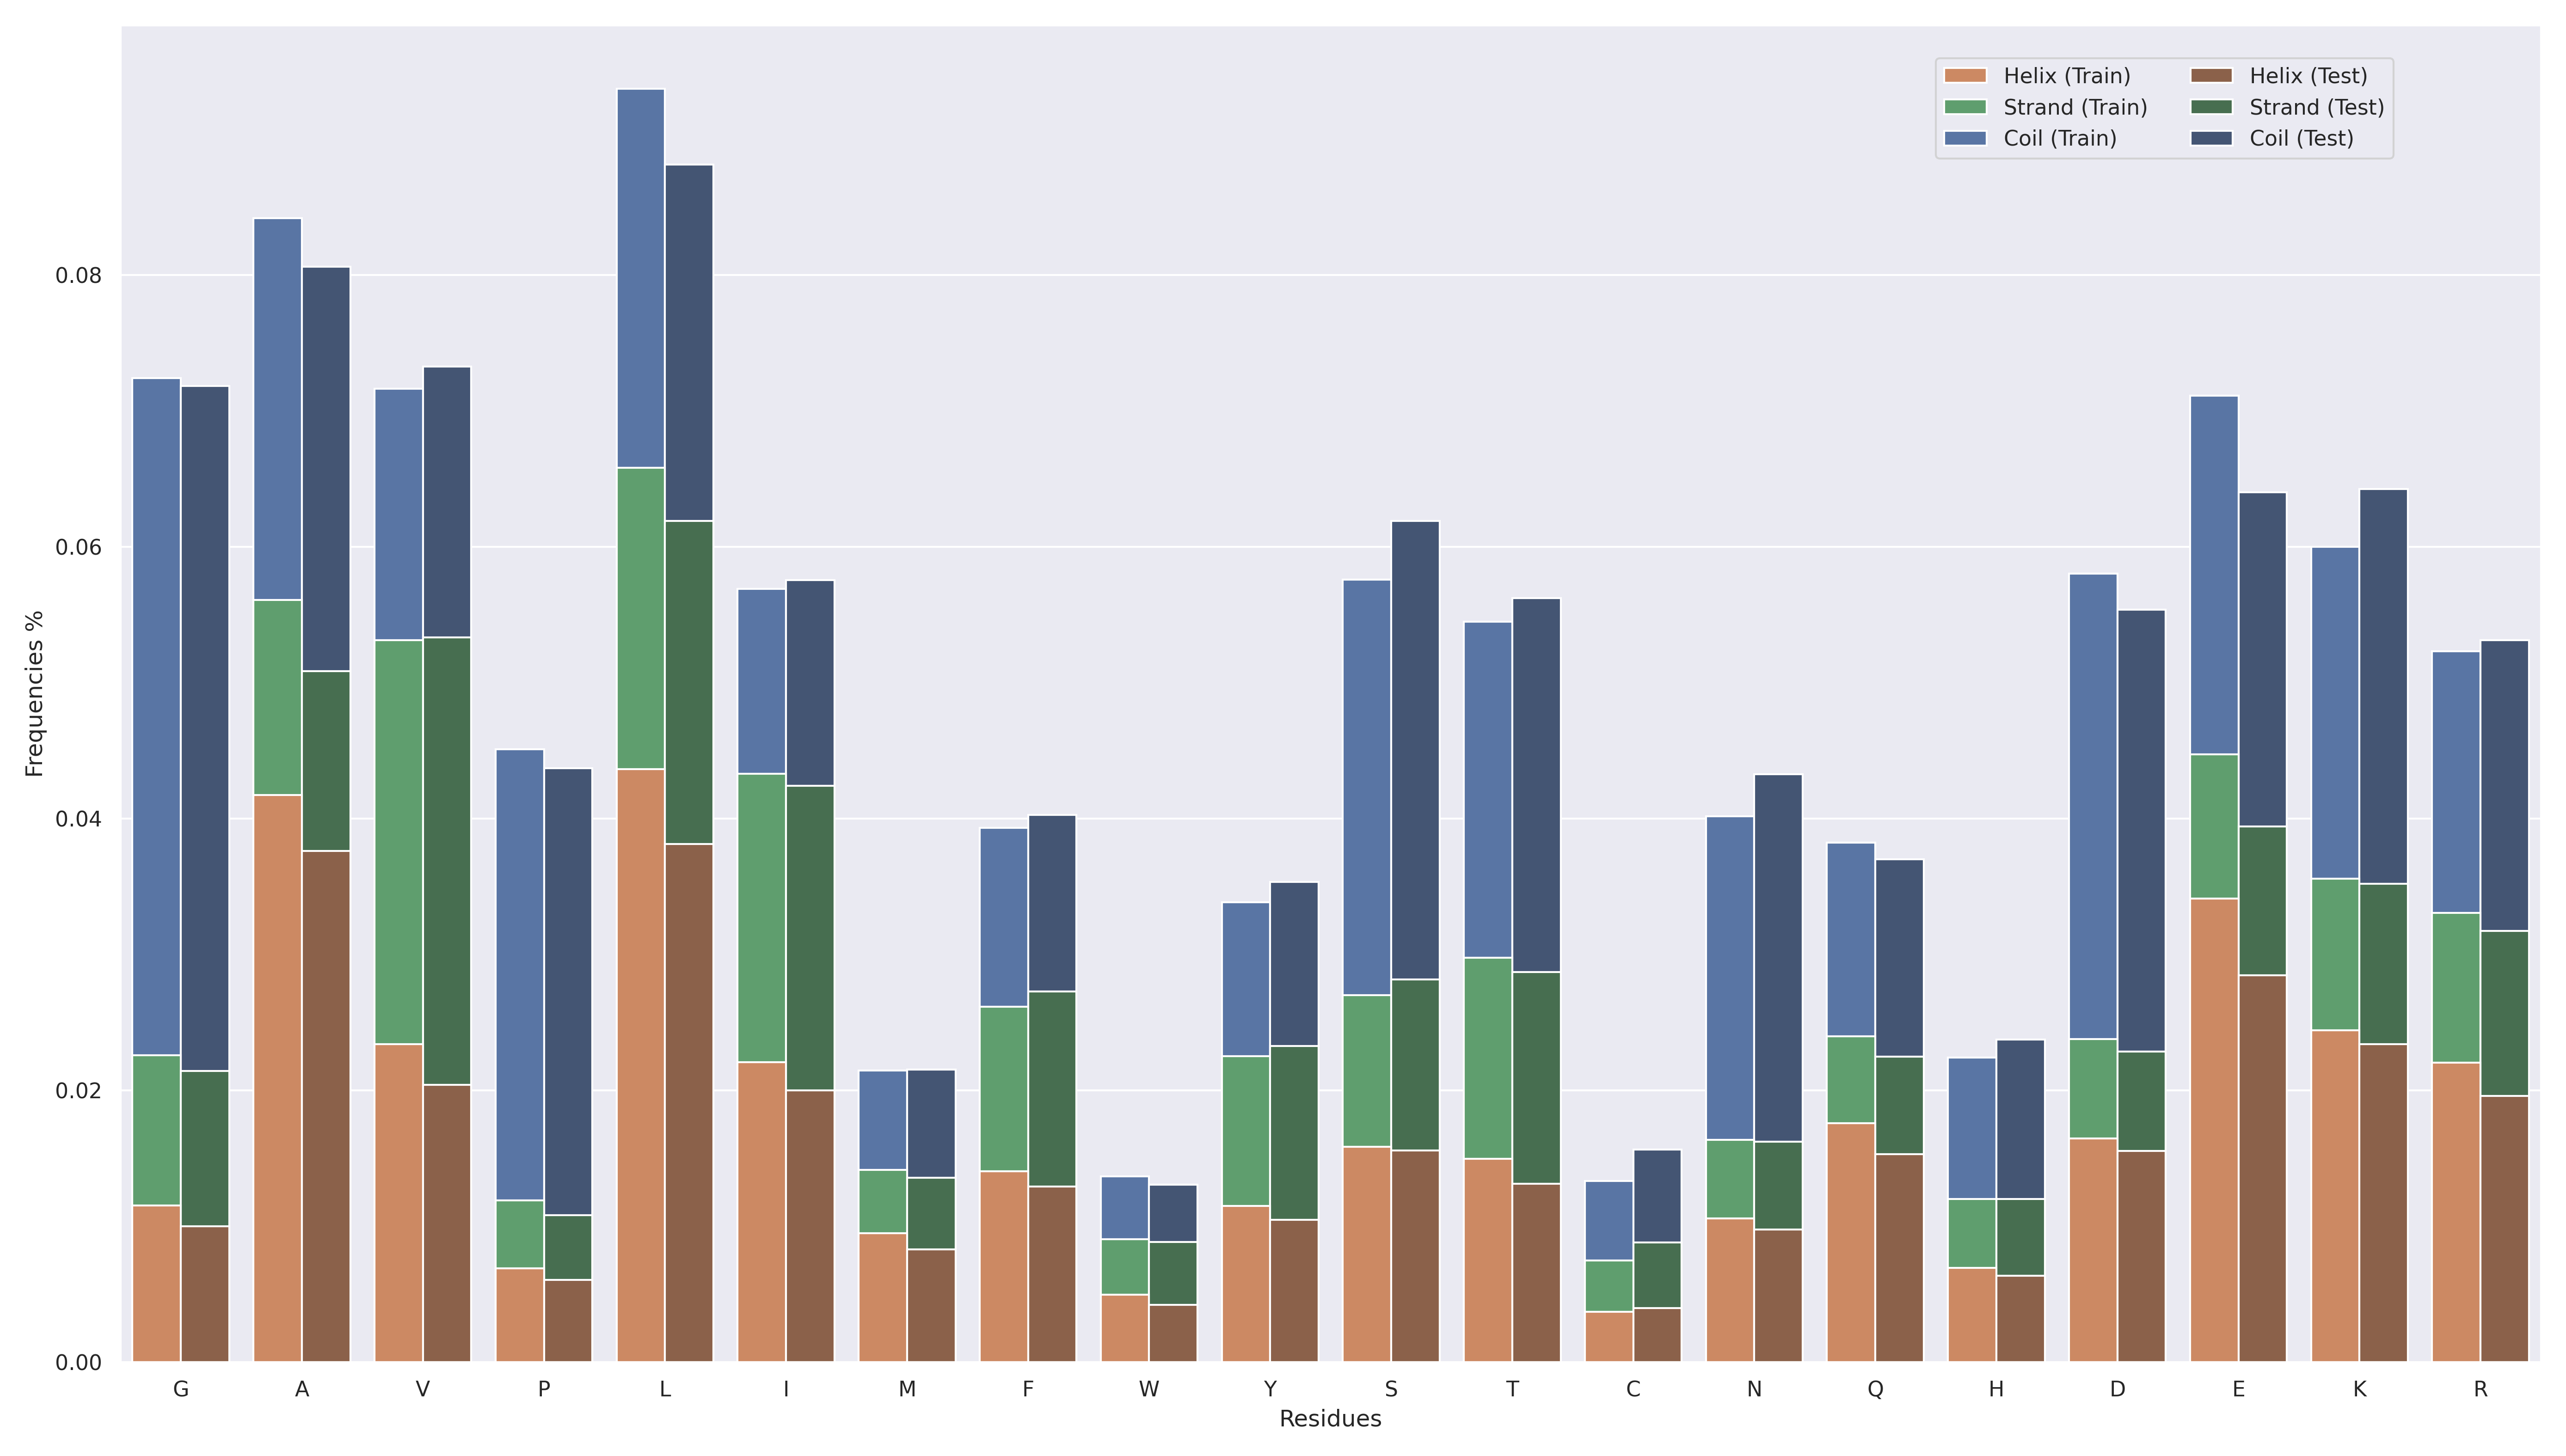
\includegraphics[width=\textwidth]{fraction_ss.png}
	\caption{Secondary structure composition on a per-residue level between train and test.}\label{fig:frac_ss}
\end{figure*}
\section{Results}
\subsection*{Dataset composition}
Great effort was taken in order to mimic the features of the original test size from JPred as close as possible.
The distribution of sequence length (\autoref{fig:seq_length}) along with the relative abundance of residues per secondary structure (\autoref{fig:frac_ss}) were consistent between training, testing and Uniprot Swiss-Prot.
Most notably, the three distributions all have the same shape, with a peak at around 100 residues and a more pronounced decay starting just before 300 residues.
\autoref{fig:frac_ss} shows how, besides a modest sampling noise, train and test sets are comparable to one another.
The proportions of classes \autoref{fig:ss_perc} between train and test sets are very comparable, thanks to the introduction of iterative resampling discussed above.

\begin{figure*}[!tb]
	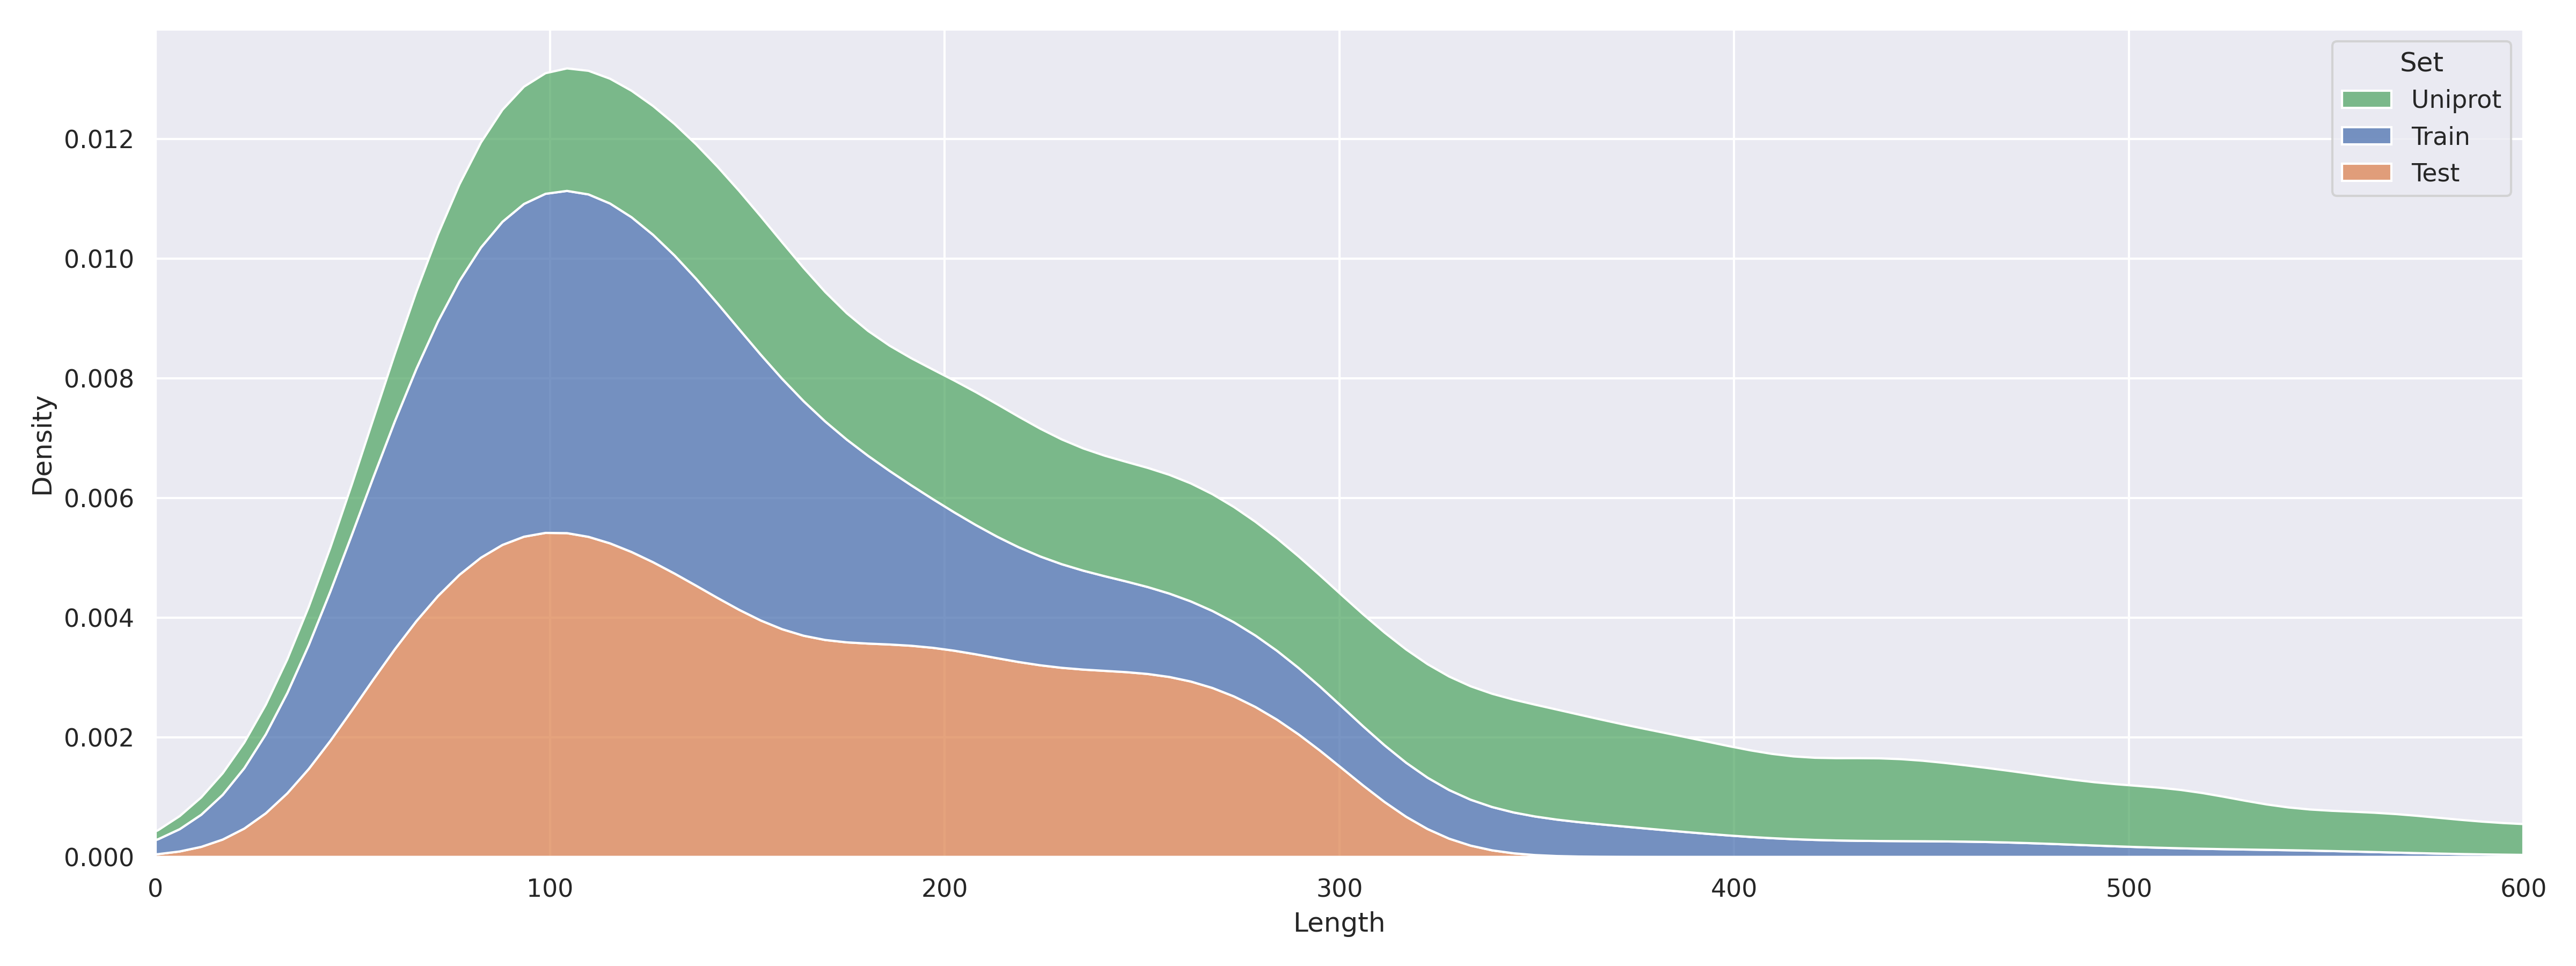
\includegraphics[width=\textwidth]{sequence_length.png}
	\caption{Sequence length comparison between train, test and Uniprot Swiss-Prot datasets.}\label{fig:seq_length}
\end{figure*}
\begin{figure}[!tb]
	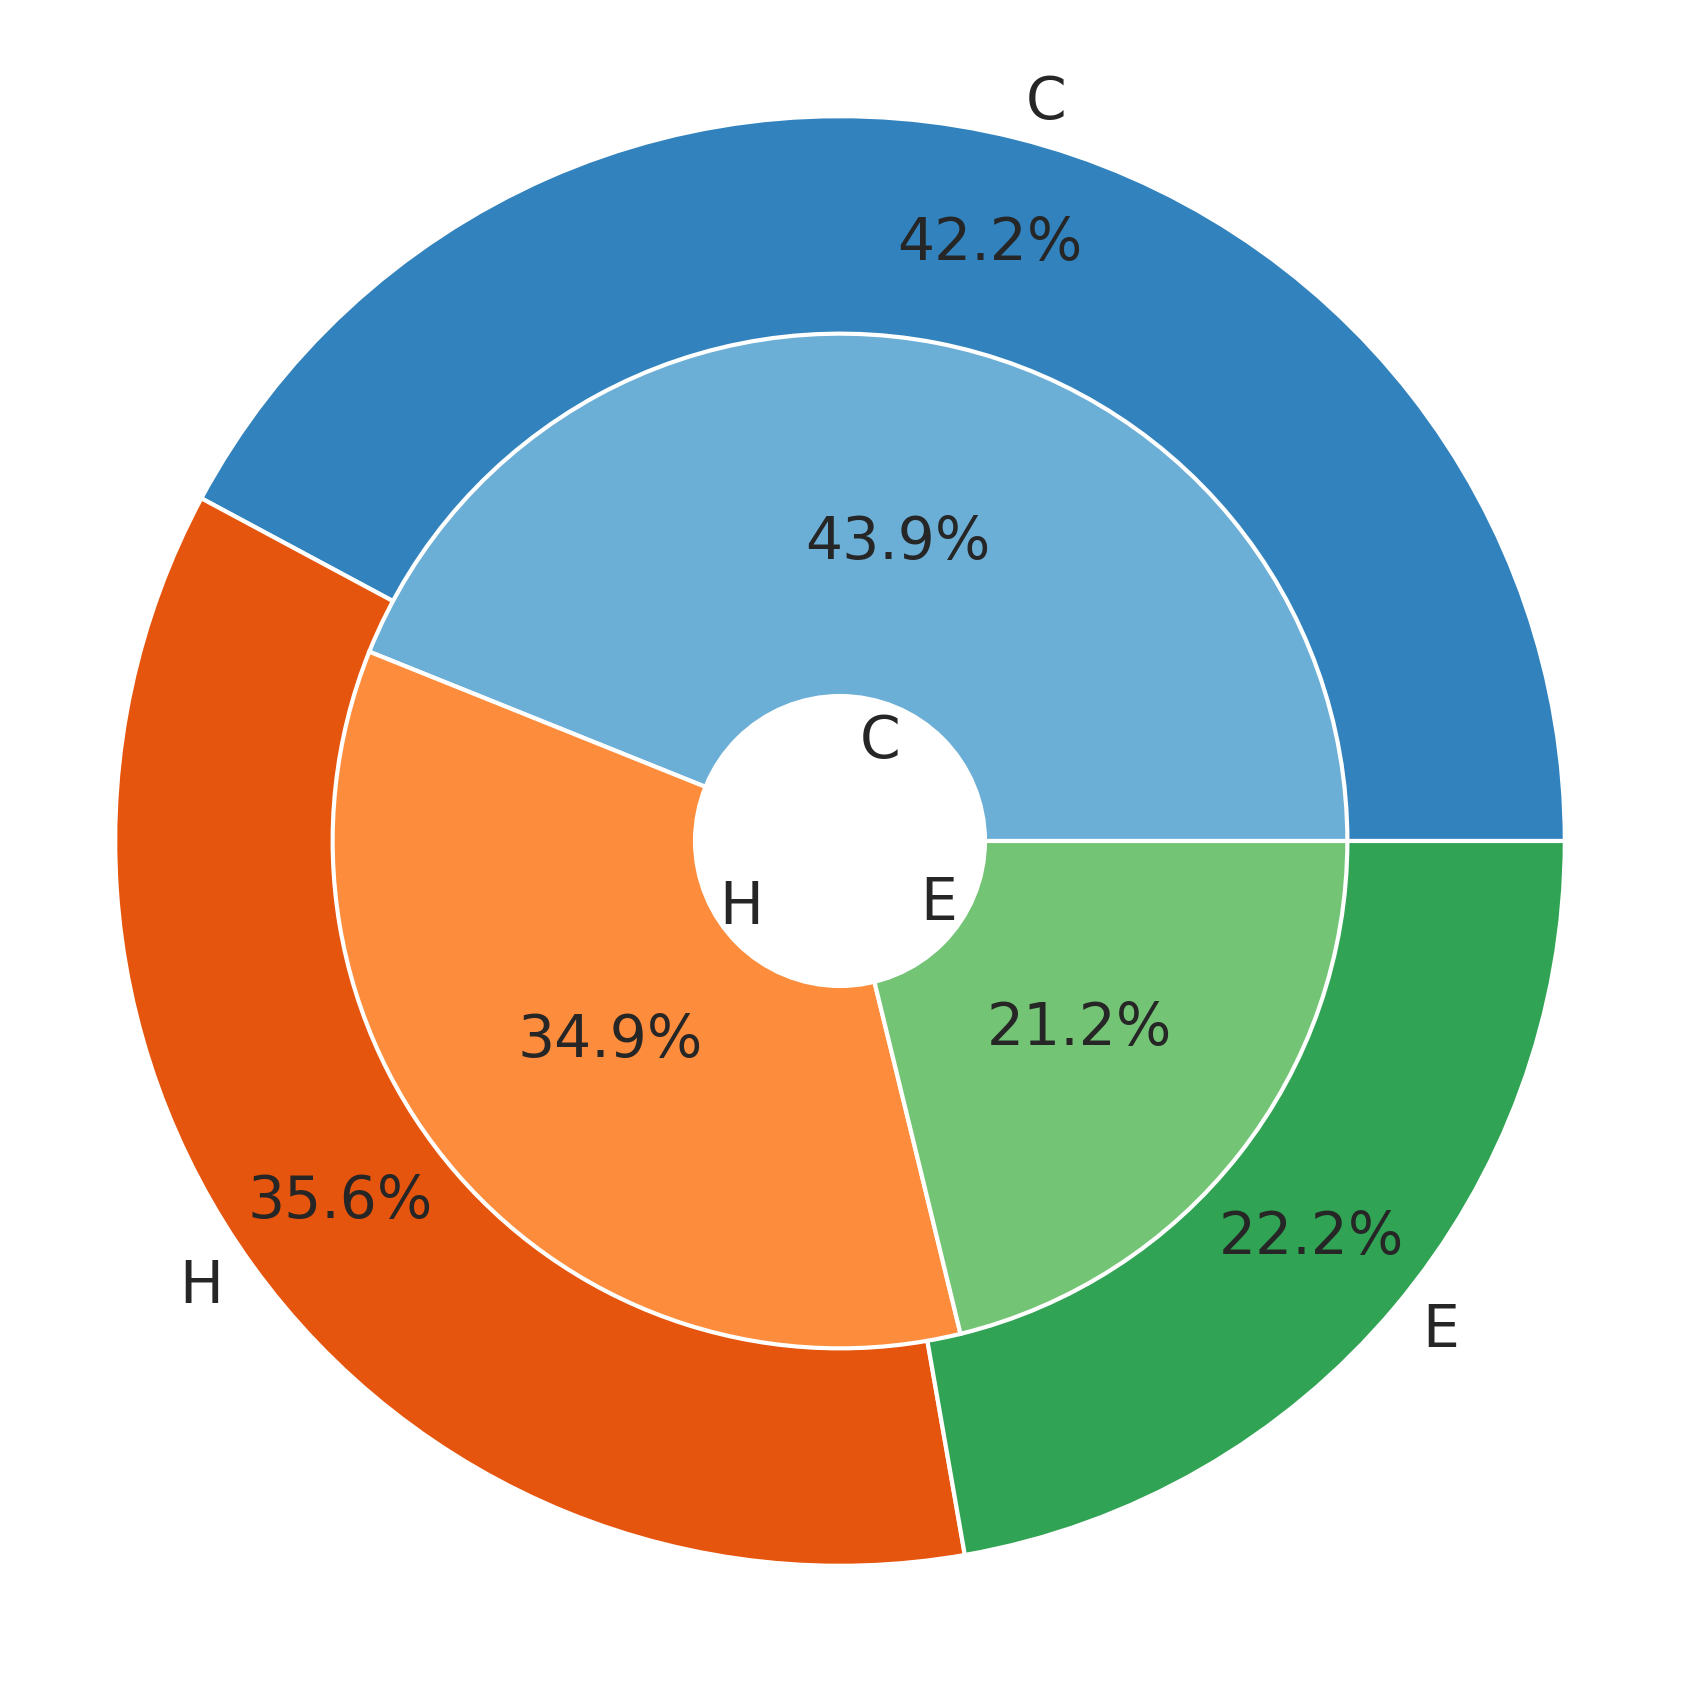
\includegraphics[width=\columnwidth]{secondary.png}
	\caption{Secondary structure comparison between train and test sets.}\label{fig:ss_perc}
\end{figure}

\subsection*{GOR}
Both models performed as expected, with a respective $Q_3$ accuracy of 0.50 and 0.63 (\autopageref{tab:q3}).
The difference between the results with when no context was given (\autoref{tab:gor_cv_w1}) and when the window was set to 17 (\autoref{tab:gor_test})  clarifies the importance and influence of nearby residues in determining the secondary structure.
The 5-fold cross validation results of the contextualized model (\autoref{tab:gor_cv}) clearly dismisses the possibility of any particular skew that may have been introduced by the training subsampling. 
Performance-wise, the MCC reported both during cross validation and testing (\autoref{tab:gor_test}) once again confirms the adequate capabilities of the GOR method to predict secondary structures despite its simplifying assumptions.
All the other metrics tell a similar story, with the notable exception of the precision of the Coil conformation.
That is, when predicting the C class the estimator has the highest confidence (high precision), even though it rarely does so (low recall).
This can be ascribed to a multitude of variables: perhaps, a fraction of the collapsed secondary structures have a very distinctive signal that triggers the estimator, either by lowering the probabilities for H and E or by incresing the one for C (or both).
This hypothesis is in line with the nature of the hybrid nature of the C class.
Without additional data we can only speculate.

The more structured nature of the helix is reflected also in the scores: it is consistently better predicted among all three.
In particular, the high recall and precision for the helix is a direct consequence of this structure's signature.
The fact that most of the information for the helix tends to fall within the window, again, is quite evident.
The same applies for the Elongated class, but in reverse.
It is known the $\beta$-bridges are more than often determined by residues quite far apart, which clearly tend not to be represented inside the window.

To no surprise, the worst overall performance belongs to the Coil class.
The reason for this outcome can be pinpointed to both the reduced mapping representation, which contributes to increase noise of its information matrix; and to the intrinsic unstructured nature of this class, which together lead wrong parameter estimation.


\subsection*{SVM}

Train (\autoref{tab:grid_train}) and test (\autoref{tab:grid_test}) scores for the grid search give valuable insights of the nuances between different kernels.
The polynomial and RBF kernels manage to achieve train scores up to 99\% across all classes, only to be significantly downsized when presented with new samples.
Nevertheless, their overfitted performance still managed to surpass the GOR model.
On the other hand, the linear and sigmoidal kernels show little differences between training and testing performance.
The latter, however, performed significantly more poorly than all the others; even worse, both train and test performances fell well below what was showed for the GOR model.
Moreover, a significant drop in score was observed for higher $\gamma$ values, which once more hints that a non-linear approach may not the right way to proceed.
All in all, it is difficult to elect a clear winner, since all the non-dismal kernels scored around 0.55 MCC.
But looking solely at the numbers, the best estimator chosen to be retrained on the whole dataset was the linear kernel.

\subsubsection*{Test}
The results of the generalization error of the best estimator were largely expected.
For an out-of-the-box SVM, out classifier managed to achieve a score of 0.73 (\autoref{tab:q3}), which is quite impressive given the minimal amount of optimization involed.
The SVM model consistently outperformed the GOR model in all scores, if not for the Helix recall and Coil precision (table \autoref{tab:svm_test}).
It seems that the SVM traded some of the precision for a significant boost in Coil recall.
Almost the same trend discussed before was observed now: the Helix class still is the easier to predict, but the Elongated and Coil classes frequently exchange places according to the metric used.
Coil precision and recall are better that Elongated, but for accuracy the situation is reversed.
However, the is a clear difference on a per-class level between the probabilistic approach of the GOR and the less transparent one of the SVM.
If before a standard error of more than 0.1 was frequently observed, right now the OvR mean show a remarkable decrease of variability between the classes.
We can suspect that this is due to the notion, or better lack thereof, that SVMs treats all numbers equally in spite of the clear biological differences that exist between them.
\begin{table}[!tbh]
	\centering
	\processtable{$Q_3$ test accuracy summary. \label{tab:q3}}{
	\begin{tabular}{lccc}
		\toprule  & GOR-1 & GOR-17 & SVM\\
		\midrule $Q_3$&\num{0.5038219235615288} &\num{0.6273162606704143} &\num{0.7302519258796586}\\
		\botrule 
\end{tabular}
}
	{}
\end{table}


\section{Discussion}
One of the most striking result is the cross validation of the second GOR model.
It clearly indicates how the model, even with the modest size of our training set, is saturated with information: no conceivable difference was noted across all five validation folds.
It's clear that the modest performances noted are, without a shadow of a doubt, direct implications of the  limitations induced by the three simplifications previously discussed.
The underlying available probabilities are correctly estimated, but the lack of predictive power resides in the approximations used to extract the information from the trained parameters.
In other words, the lack of complexity constrains the model to pick up only the most evident patterns: helix and strands.
Moreover, the paramount importance of the sequence context is confirmed by the sub-par performance of the context-deprived estimator ()\autoref{tab:q3}).
In synthesis, the gor model trained is as good as it can get (* GOR V accounts for residues pairs and triplets, decision constants in the final prediction, 13 residues window); to achieve higher performances there is the need to look for other approaches.
In this regard, the SVM classifier consistently outperformed the GOR method, but this has to be expected since it encapsulates decades of machine learning advancements.
The possibility to model non-linearity, introduced by non-linear functions, was a great achievement.
Unfortunately, our results show that this feature of SVMs was not necessary to achieve satisfactory performances.
Both the influence of the $\gamma$ parameter and, perhaps surprisingly, the use of non linear kernels clearly were not rewarded.
To be fair, the performance differences between the linear and non-linear kernels were not that obvious, but the noticeable tendency to overfitting, for the non-linear kernels, should come at least as suspicious.
In summary, SVMs, when properly optimized, can offer a consistent boost in performance with respect to their probabilistic counterparts.
However, careful hyperparameter optimization is needed to achieve satisfactory results; a not so trivial use-case given their problem dependence.
Moreover, the fact that they are more or less "black boxes" makes it difficult to derive biological knowledge, even from well fitted estimators.
This remark can be juxtaposed to the notion that a deep understanding of the biological reality is perhaps even more important than the sheer power of the model.
Such consideration inspired by the stunning effect of the sequence context in the accuracy for the model performance.
More powerful and efficient models (i.e. neural networks) have been proven to work nearby the theoretical upper limit.
As of today, it is difficult to recommend  support vector machines for secondary structure prediction, at least with their naive implementation.


%\bibliographystyle{natbib}
%\bibliographystyle{achemnat}
%\bibliographystyle{plainnat}
%\bibliographystyle{abbrv}
%\bibliographystyle{bioinformatics}
%
%\bibliographystyle{plain}
%
%\bibliography{Document}

\bibliographystyle{natbib}
\bibliography{./references.bib}


\begin{supplementary}
	\section*{Supplementary material}


	\begin{table}[h]		
		\processtable{GOR method train and test MCC.\label{tab:gor_cv}}{
			\begin{tabular}{lrrrrrr}
				\toprule Fold  &    1 &    2 &    3 &    4 &    5 & Average \\
				\midrule
				Train score & \num{0.46717477} &\num{ 0.46827731} & \num{0.47621793} & \num{0.46023879} & \num{0.46305542} & \num{0.466992844}$\pm$\num{0.0027194274661472414} \\
				Test score	 & \num{0.47218079} & \num{0.46993699} & \num{0.46430272} & \num{0.47239888}& \num{0.46637996} & \num{0.469039868}$\pm$\num{0.0016041954720588184} \\
				\botrule
			\end{tabular}
		}
		{}

	\processtable{MCC train scores for the grid search of the SVM.\label{tab:grid_train}} {
	\centering
	\begin{tabular}{lllrrrrrrr}
		\toprule
Fold
		&   &     &              1 &              2 &              3 &              4 &              5 &        Average\\
		Kernel & $C$ & $\gamma$ &                &                &                &                &                &                &                \\
		\midrule
		\multirow{2}{*}{linear} & 2 & NA & \num{0.555878} & \num{0.553829} & \num{0.552153} & \num{0.557738} & \num{0.557615} & \num{0.555443}$\pm$\num{0.001086} \\
		& 4 & NA & \num{0.555992} & \num{0.554007} & \num{0.552000} & \num{0.557634} & \num{0.557678} & \num{0.555462}$\pm$\num{0.001096} \\
		\cline{1-10}
		\multirow{4}{*}{polynomial} & \multirow{2}{*}{2} & 0.5 & \num{0.990789} & \num{0.991195} & \num{0.991465} & \num{0.992246} & \num{0.991366} & \num{0.991412}$\pm$\num{0.000238} \\
		&   & 2.0 & \num{0.994878} & \num{0.994546} & \num{0.995161} & \num{0.995797} & \num{0.995600} & \num{0.995196}$\pm$\num{0.000229} \\
		\cline{2-10}
		& \multirow{2}{*}{4} & 0.5 & \num{0.993187} & \num{0.993403} & \num{0.993633} & \num{0.994434} & \num{0.993793} & \num{0.993690}$\pm$\num{0.000212} \\
		&   & 2.0 & \num{0.994878} & \num{0.994546} & \num{0.995161} & \num{0.995797} & \num{0.995600} & \num{0.995196}$\pm$\num{0.000229} \\
		\cline{1-10}
		\cline{2-10}
		\multirow{4}{*}{rbf} & \multirow{2}{*}{2} & 0.5 & \num{0.977874} & \num{0.978645} & \num{0.978895} & \num{0.979353} & \num{0.979207} & \num{0.978795}$\pm$\num{0.000261} \\
		&   & 2.0 & \num{0.994452} & \num{0.994223} & \num{0.994718} & \num{0.995432} & \num{0.995130} & \num{0.994791}$\pm$\num{0.000220} \\
		\cline{2-10}
		& \multirow{2}{*}{4} & 0.5 & \num{0.990191} & \num{0.990466} & \num{0.990577} & \num{0.991169} & \num{0.990650} & \num{0.990611}$\pm$\num{0.000160} \\
		&   & 2.0 & \num{0.994842} & \num{0.994545} & \num{0.995150} & \num{0.995788} & \num{0.995565} & \num{0.995178}$\pm$\num{0.000228} \\
		\cline{1-10}
		\cline{2-10}
		\multirow{4}{*}{sigmoid} & \multirow{2}{*}{2} & 0.5 & \num{0.328678} & \num{0.299505} & \num{0.291998} & \num{0.301405} & \num{0.298406} & \num{0.303998}$\pm$\num{0.006369} \\
		&   & 2.0 & \num{0.152810} & \num{0.084148} & \num{0.098710} & \num{0.000000} & \num{0.062155} & \num{0.079565}$\pm$\num{0.024886} \\
		\cline{2-10}
		& \multirow{2}{*}{4} & 0.5 & \num{0.298454} & \num{0.300317} & \num{0.292689} & \num{0.301721} & \num{0.298623} & \num{0.298361}$\pm$\num{0.001539} \\
		&   & 2.0 & \num{0.000000} & \num{0.104535} & \num{0.098752} & \num{0.065581} & \num{0.062111} & \num{0.066196}$\pm$\num{0.018613} \\
		\botrule
	\end{tabular}
}{ciaociao}

\vspace{8pt}
\processtable{MCC test scores for the grid search of the SVM.\label{tab:grid_test}} {
	\begin{tabular}{lllrrrrrrr}
		\toprule
Fold
		&   &     &              1 &              2 &              3 &              4 &              5 &        Average \\
		Kernel & $C$ & $\gamma$ &                &                &                &                &                &                &                \\
		\midrule
		\multirow{2}{*}{linear} & 2 & NA & \num{0.548214} & \num{0.550551} & \num{0.566465} & \num{0.543312} & \num{0.544310} & \num{0.550570}$\pm$\num{0.004184} \\
		& 4 & NA & \num{0.547902} & \num{0.550680} & \num{0.566574} & \num{0.543056} & \num{0.544325} & \num{0.550507}$\pm$\num{0.004235} \\
		\cline{1-10}
		\multirow{4}{*}{polynomial} & \multirow{2}{*}{2} & 0.5 & \num{0.543048} & \num{0.544112} & \num{0.555780} & \num{0.539354} & \num{0.533803} & \num{0.543220}$\pm$\num{0.003621} \\
		&   & 2.0 & \num{0.496472} & \num{0.504056} & \num{0.513664} & \num{0.497487} & \num{0.488898} & \num{0.500116}$\pm$\num{0.004154} \\
		\cline{2-10}
		& \multirow{2}{*}{4} & 0.5 & \num{0.526062} & \num{0.528195} & \num{0.542334} & \num{0.523454} & \num{0.518509} & \num{0.527711}$\pm$\num{0.003997} \\
		&   & 2.0 & \num{0.497074} & \num{0.504222} & \num{0.514401} & \num{0.497302} & \num{0.488238} & \num{0.500248}$\pm$\num{0.004354} \\
		\cline{1-10}
		\cline{2-10}
		\multirow{4}{*}{rbf} & \multirow{2}{*}{2} & 0.5 & \num{0.549098} & \num{0.552093} & \num{0.560020} & \num{0.538876} & \num{0.540715} & \num{0.548160}$\pm$\num{0.003864} \\
		&   & 2.0 & \num{0.168477} & \num{0.185074} & \num{0.184087} & \num{0.168964} & \num{0.153202} & \num{0.171961}$\pm$\num{0.005882} \\
		\cline{2-10}
		& \multirow{2}{*}{4} & 0.5 & \num{0.538637} & \num{0.544823} & \num{0.549845} & \num{0.529817} & \num{0.530986} & \num{0.538822}$\pm$\num{0.003873} \\
		&   & 2.0 & \num{0.166752} & \num{0.181849} & \num{0.181077} & \num{0.166299} & \num{0.150768} & \num{0.169349}$\pm$\num{0.005723} \\
		\cline{1-10}
		\cline{2-10}
		\multirow{4}{*}{sigmoid} & \multirow{2}{*}{2} & 0.5 & \num{0.322609} & \num{0.301769} & \num{0.324009} & \num{0.298731} &\num{0.302430} & \num{0.309910}$\pm$\num{0.005510} \\
		&   & 2.0 & \num{0.148171} & \num{0.063996} & \num{0.107723} & \num{0.000000} & \num{0.069370} & \num{0.077852}$\pm$\num{0.024660} \\
		\cline{2-10}
		& \multirow{2}{*}{4} & 0.5 & \num{0.307181} & \num{0.302182} & \num{0.323896} & \num{0.298461} & \num{0.301903} & \num{0.306724}$\pm$\num{0.004512} \\
		&   & 2.0 & \num{0.000000} & \num{0.087364} & \num{0.107763} & \num{0.048488} & \num{0.069351} & \num{0.062593}$\pm$\num{0.018461} \\
		\bottomrule
	\end{tabular}
}
{}

	\processtable{GOR estimato metrics with window size set to 1.\label{tab:gor_cv_w1}}{
	\begin{tabular}{lrrrr}
		\toprule
		{} &              Helix &              Elongated &              Coil &            OvR             \\
		\midrule
		Precision                        & \num{0.491961} & \num{0.362587} & \num{0.631006} & \num{0.495185}$\pm$\num{0.077503} \\
		Recall                           & \num{0.468362} & \num{0.506214} & \num{0.531024} & \num{0.501866}$\pm$\num{0.018219} \\
		Accuracy                         & \num{0.646199} & \num{0.700714} & \num{0.660731} & \num{0.669215}$\pm$\num{0.016299} \\
		Matthews Correlation Coefficient & \num{0.212189} & \num{0.233705} & \num{0.300192} & \num{0.248695}$\pm$\num{0.026487} \\
		\bottomrule
	\end{tabular}
}
{}
	\processtable{GOR estimator blind set metrics with window size set to 17.\label{tab:gor_test}} {

\begin{tabular}{lrrrr}
	\toprule
Score
	{} &              Helix &              Elongated &              Coil &            OvR  \\
	\midrule
	Precision                        & \num{0.641402} & \num{0.469575} & \num{0.826408} & \num{0.645795}$\pm$\num{0.103032} \\
	Recall                           & \num{0.803627} & \num{0.734224} & \num{0.435615} & \num{0.657822}$\pm$\num{0.112895} \\
	Accuracy                         & \num{0.774641} & \num{0.768020} & \num{0.711972} & \num{0.751544}$\pm$\num{0.019878} \\
	Matthews Correlation Coefficient & \num{0.540730} & \num{0.443918} & \num{0.428262} & \num{0.470970}$\pm$\num{0.035171} \\
	\bottomrule
\end{tabular}
}
{}	


\processtable{SVM estimator blind set metrics\label{tab:svm_test}} {	
\begin{tabular}{lrrrr}
	\toprule
	{} &              Helix &              Elongated &              Coil &            OvR\\
	\midrule
	Precision                        & \num{0.766918} & \num{0.681765} & \num{0.722560} & \num{0.723748}$\pm$\num{0.024589} \\
	Recall                           & \num{0.739561} & \num{0.571063} & \num{0.799640} & \num{0.703421}$\pm$\num{0.068414} \\
	Accuracy                         & \num{0.830648} & \num{0.852675} & \num{0.777181} & \num{0.820168}$\pm$\num{0.022414} \\
	Matthews Correlation Coefficient & \num{0.624449} & \num{0.534157} & \num{0.555296} & \num{0.571301}$\pm$\num{0.027266} \\
	\bottomrule
\end{tabular}
}
{The results refer to an estimator trained on the whole training set with a linear kernel, C set to 2 and $\gamma$ set to 0.5.}
\end{table}

\begin{figure}
	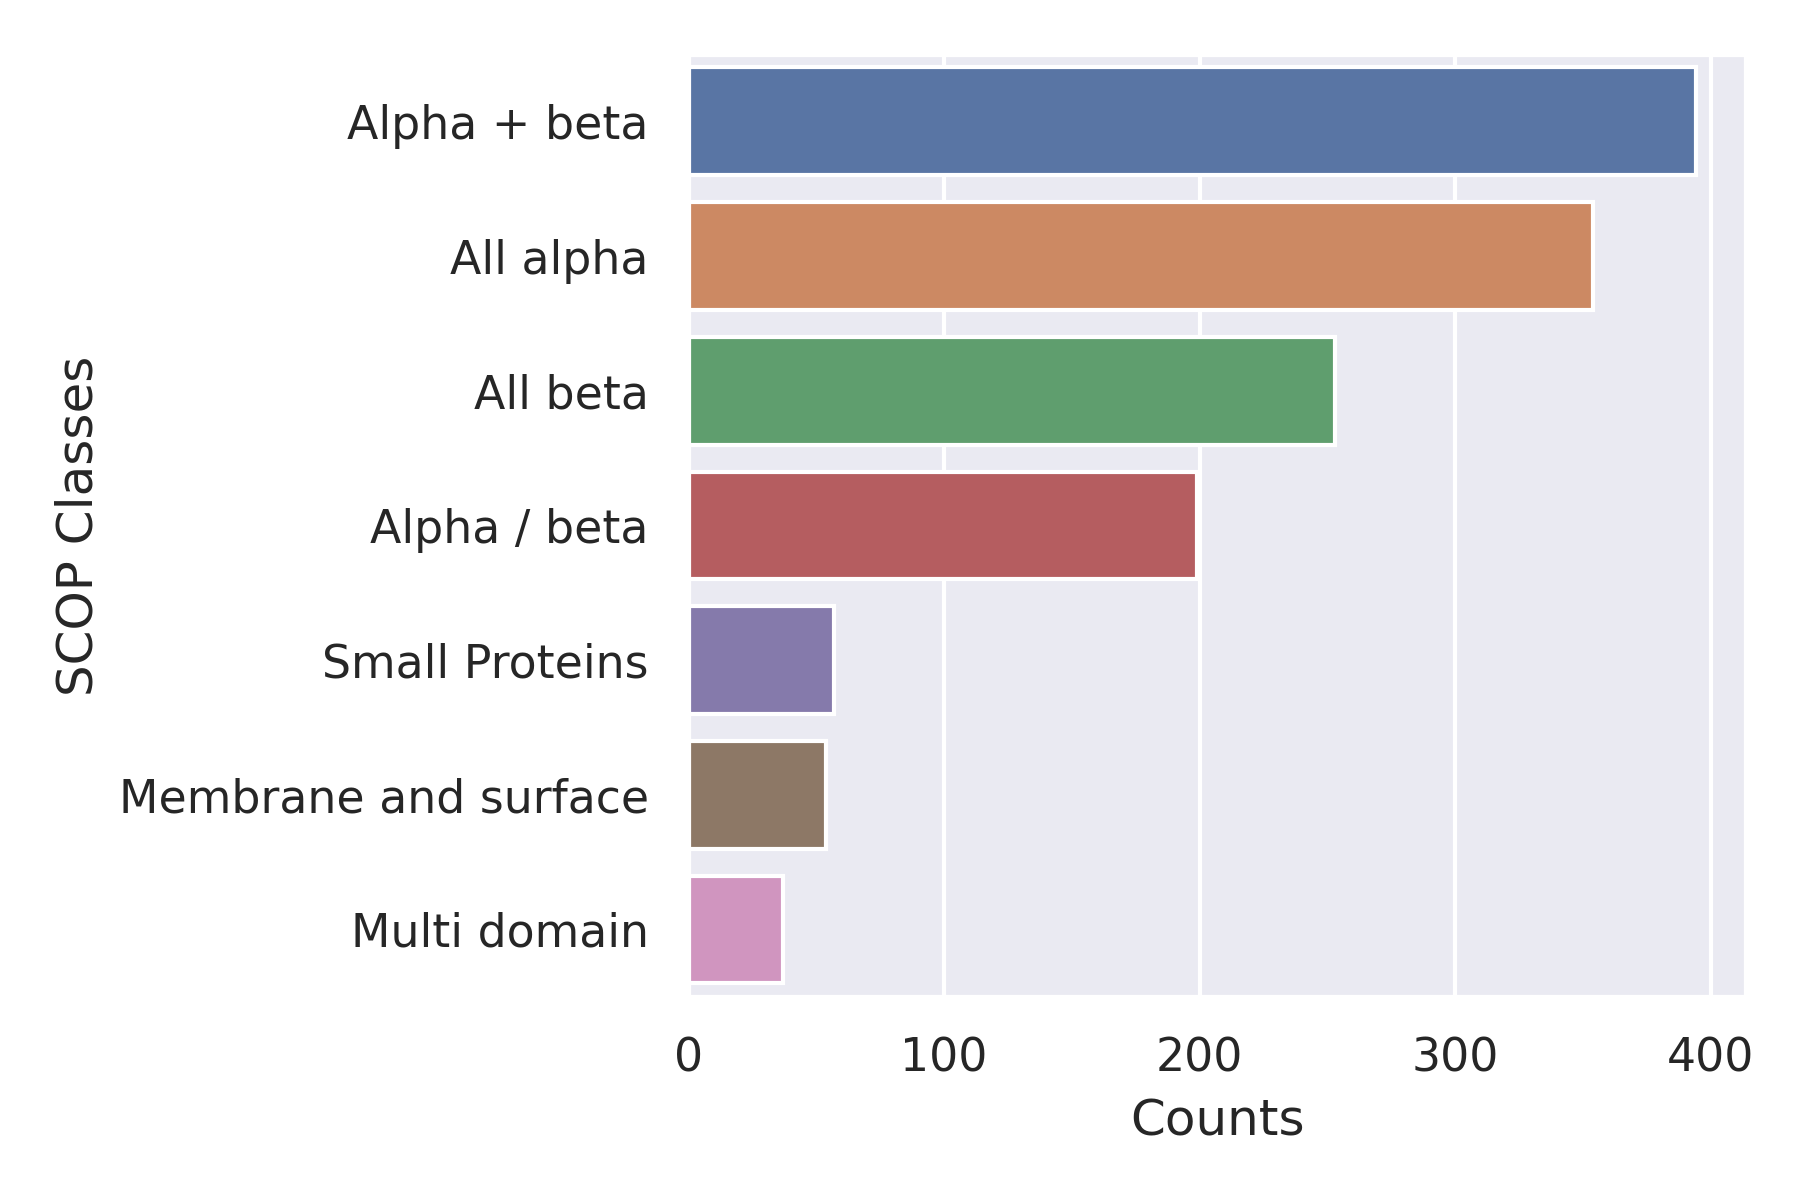
\includegraphics[width=\textwidth]{scop.png}
	\caption{Sequence length comparison between train, test and Uniprot Swiss-Prot datasets.}\label{fig:seq_length}
\end{figure}
\end{supplementary}
\end{document}
